\subsection{Variaci\'on de la resistencia $R_8$}

\paragraph*{Influencia en la funci\'on transferencia:} A continuaci\'on se muestra la funci\'on transferencia del circuito, con $R_8\to 0$ y luego con $R_8\to \infty$. Para ambos casos se obtiene la expresi\'on en funci\'on del resto de los componentes del circuito y se agrega el resultado luego de reemplazar dichas expresiones con los valores de los componentes empleados (indicados en la tabla \ref{componentes}.

\begin{equation}
\lim_{R_8\to 0} H(s) = - \frac{R_4 + R_5}{R_5} \cdot 
\left(\frac{C_2 C_6 R_1 R_3 R_5 R_7}{C_6 R_6 R_7(R_4 + R_5)+\frac{R_4 R_5}{C_2 C_6 R_1 R_3 (R_4+R_5)}}\right)s = - 9.63 \cdot 10^{-13} s
\end{equation}

\begin{equation}
\lim_{R_8\to \infty} H(s) = \frac{R_4 + R_5}{R_5} \cdot \frac{s^2 + \frac{1}{C_6 R_7}s}{s^2 + \frac{R_6 + R_7}{C_6 R_6 R_7}\cdot s + \frac{R_4}{C_2 C_6 R_1 R_3 R_5}} = \frac{1.59 s^{2} + 4473.45}{s^{2} + 6699.83 s + 104,39 \cdot 10^6}
\end{equation}

Se pueden ver en el siguiente gr\'afico la funci\'on transferencia para estos dos casos.

\begin{figure}[H] %!ht
	\centering
	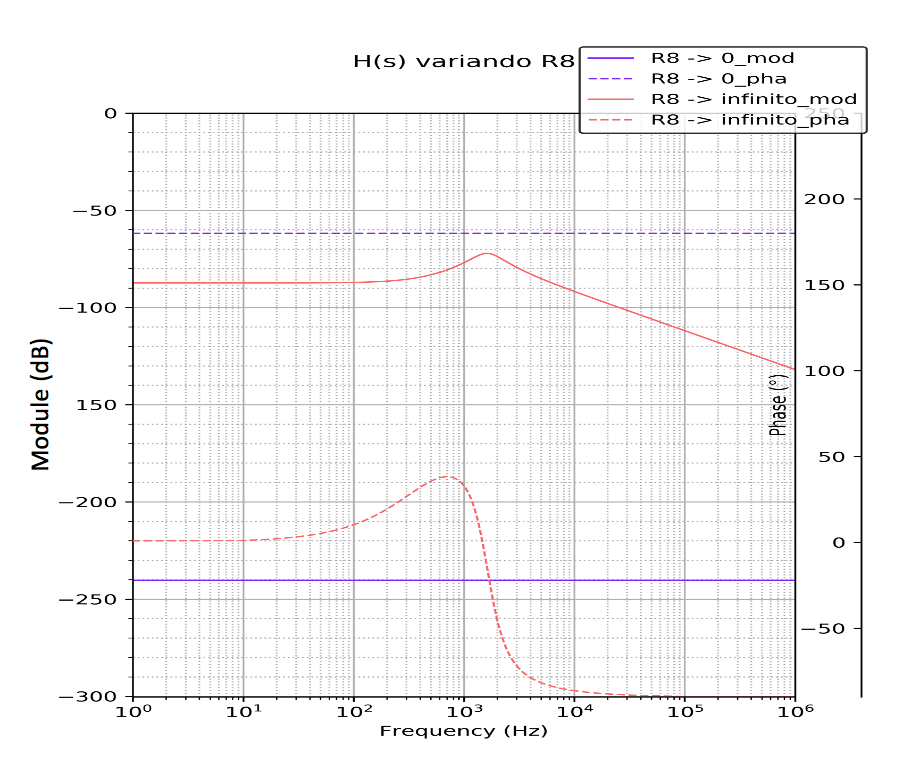
\includegraphics[width=10cm,height=10cm,keepaspectratio]{../EJ1/00GRAFICOS/r88.png}
	\caption{H(s) con $R_8 \to 0$ y $R_8 \to \infty$}
	\label{r8}
\end{figure}

Mirando la ganancia en el gr\'afico \ref{r8}, es facil notar que el valor de la resistencia $R_8$ es fundamental para el filtro high pass notch, ya que cortocircuitandola o abriendo el circuito en su lugar, el comportamiento del circuito es completamente distinto.

\subsection{Variaci\'on de la resistencia $R_6$}

A continuaci\'on se muestra c\'omo cambian los polos y ceros al modificar la resistencia $R_6$ en la expresi\'on de la transferencia \ref{vovi}, dejando fijas las otras resistencias y los capacitores con los valores determinados para implementar el filtro.


\begin{figure}[H] %!ht
	\centering
	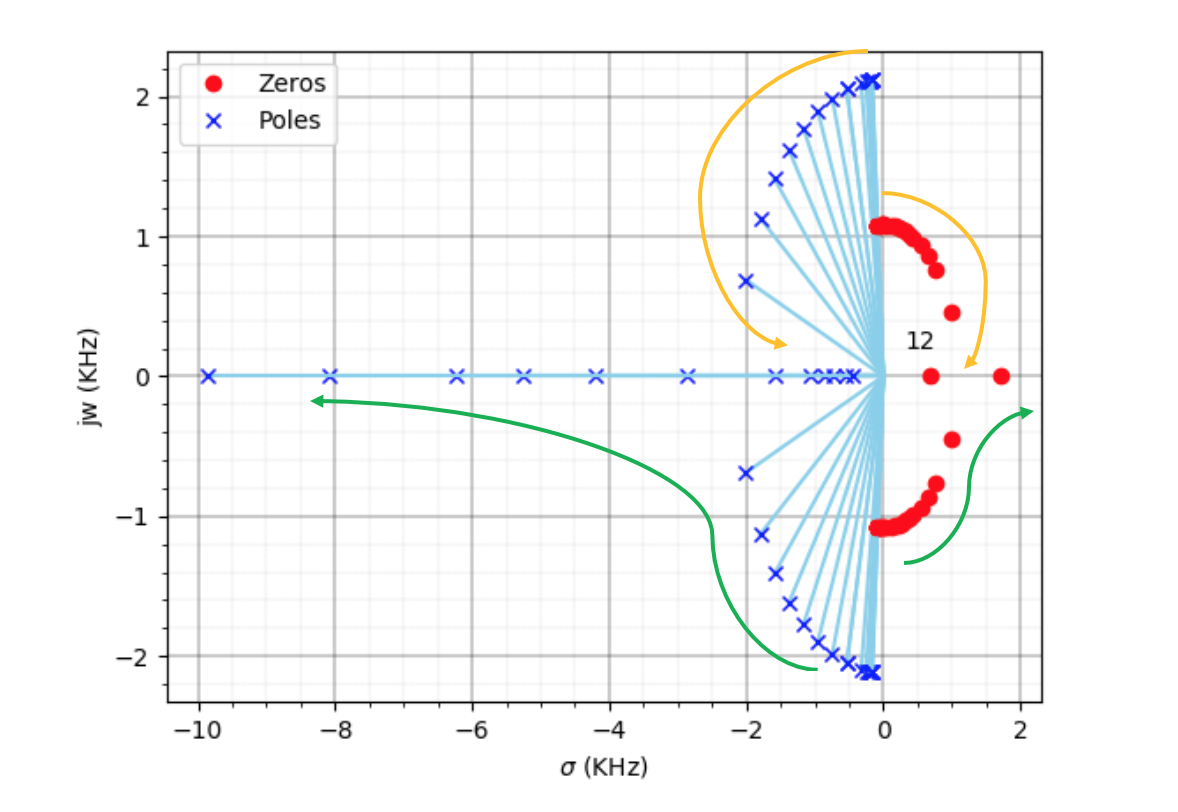
\includegraphics[width=10cm,height=10cm,keepaspectratio]{../EJ1/00GRAFICOS/r6.png}
	\caption{Polos y ceros del circuito al variar $R_6$}
	\label{r6}
\end{figure}

En la figura \ref{r6} se indica con flechas hacia donde tienden los polos y los ceros al hacer tender R6 a cero. Las flechas amarillas corresponden a la variaci\'on del polo $P1$ y del cero $Z1$ en dicho caso, mientras que las flechas verdes indican el comportamiento del polo $P2$ y del cero $Z2$. Para el caso en el que R6 tiende a infinito, las flechas van en sentido contrario al indicado en la figura. A continuaci\'on se muestran anal\'iticamente dichos comportamientos:

\begin{equation}
	\lim_{R_6\to 0} s_{z1,z2} \approx \lim_{R_6\to 0}\left( \frac{R_4 R_5}{C_6 R_6 R_8} \pm \frac{R_4 R_5}{C_6 R_6 R_8}\right) \Rightarrow 
	\begin{cases} 
	s_{z1} \to +\infty\\
	s_{z2} \to 0
	\end{cases}
\end{equation}

\begin{equation}
	\lim_{R_6\to 0} s_{p1,p2} \approx 	\lim_{R_6\to 0} \left( -\frac{R_6 + R_7}{C_6 R_6 R_7} \pm \frac{R_6 + R_7}{C_6 R_6 R_7} \right) \Rightarrow
	\begin{cases} 
	s_{p1} \to 0\\
	s_{p2} \to -\infty
	\end{cases}
\end{equation}

\begin{equation}
\lim_{R_6\to\infty}s_{z1,z2} =  -\frac{1}{C_6 R_7} \pm \sqrt{\left(\frac{1}{C_6 R_7} \right)^2 - 4 \cdot \frac{R_4 R_5}{C_2 C_6 R_1 R_3 R_8(R_4 + R_5)}}
\end{equation}

\begin{equation}
\lim_{R_6\to\infty}s_{p1,p2} =  - \frac{1}{C_6 R_7} \pm \sqrt{\left(\frac{1}{C_6 R_7}\right)^2 - 4 \cdot \frac{R_4 (R_5 + R_8)}{C_2 C_6 R_1 R_3 R_5 R_8 }}
\end{equation}

